\documentclass[12pt]{article}
\usepackage[utf8]{inputenc}
\usepackage{graphics}
\usepackage{graphicx}
\usepackage{float}
\usepackage{hyperref}
\hypersetup{
	colorlinks=true,
	linkcolor=blue,
	filecolor=magenta,      
	urlcolor=cyan,
}

\title{Ontwikkelstraat opzetten}
\author{Thomas van Dongen, Koen Schilders}
\date{14 maart 2018}

\begin{document}


% De titelpagina
\begin{titlepage}
\maketitle
\end{titlepage}

<<<<<<< HEAD
\section{Automatisch deployen}
Tijdens het opzetten van de docker opdracht hebben wij gelijk het automatisch deployen ingesteld. Hierdoor hoefde dit niet meer te gebeuren bij deze opdracht.

\section{Mail configuratie}
Om er voor te zorgen dat er mails verzonden worden is er een post-build action toegevoegd met de mail client van jenkins. 
\newline
\begin{figure}[H]
	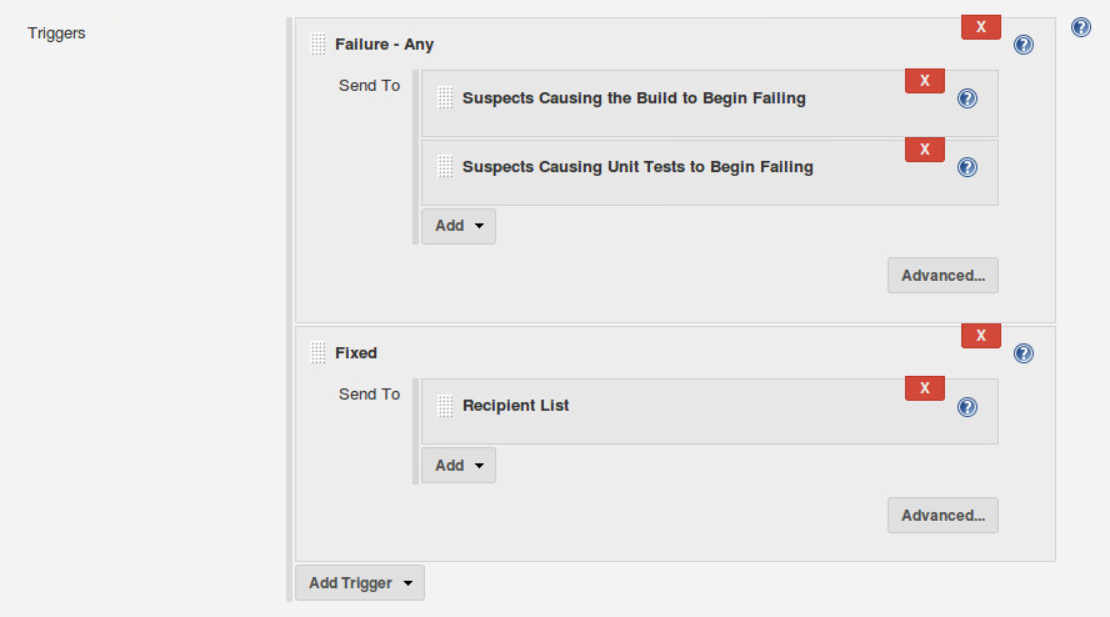
\includegraphics[width=\textwidth]{images/emailsetting.png}
	\caption{post-build jenkins configuratie\label{fig:mail_conf}}
\end{figure}

\newpage
\section{Artfactory}
Daarnaast hebben we da Artfactory plugin geinstalleerd op de jenkins docker. Om op een backup te kunnen maken van de gebuilde wars. Dit is dus ook een post-build action die we toegevoegd hebben aan jenkins.

\begin{figure}[H]
	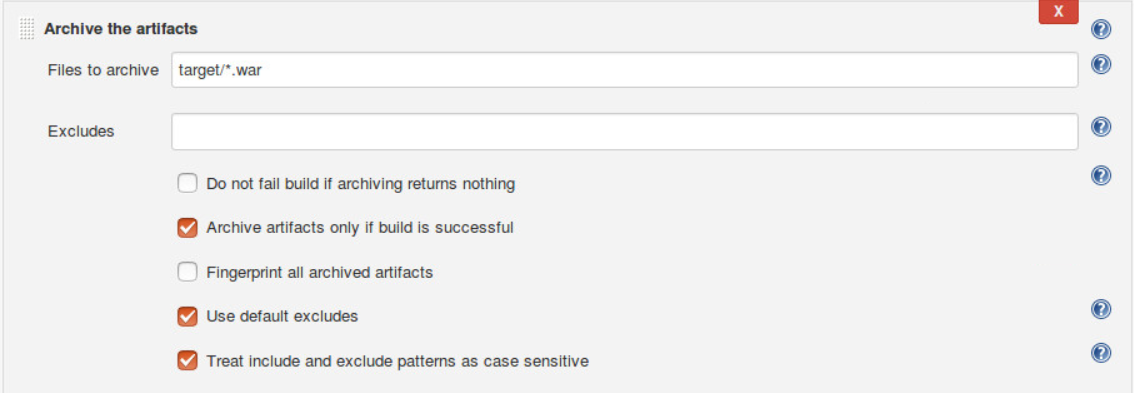
\includegraphics[width=\textwidth]{images/Archivesetting.png}
	\caption{Artfactory configuratie\label{fig:artfactory}}
\end{figure}

\section{Controle}
Om te controleren of de configuratie geholpen heeft hebben we een test gedaan met onze ontwikkelstraat. Hier was het dus de bedoeling dat de applicatie automatisch vanuit Git in onze glassfish server terecht kwam. In een screenshot hier is te zien dat de punten die in dit document vermeld zijn uitgevoerd worden.

\begin{figure}[H]
	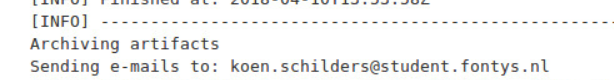
\includegraphics[width=\textwidth]{images/Archivingandsendingemails.png}
	\caption{Log van het archiveren en mailen\label{fig:log}}
\end{figure}

\newpage
\section{Conclusie}
Door deze tools toe te voegen aan jenkins hebben we nu een ontwikkelstraat opgezet die automatisch: build, test en deployed. Als er ergens iets fout gaat wordt hier naar de destbetreffende persoon een mailtje gestuurd.


\end{document}